\documentclass{article}
\usepackage[utf8]{inputenc}
\usepackage{multicol}
\usepackage{fancyhdr}
\usepackage{geometry}
\usepackage{graphicx}
\usepackage{mdframed}
\usepackage{indentfirst}
\usepackage{enumitem}
\usepackage{amsmath}
\usepackage{amsfonts}
\usepackage{mathtools}

% For code styles:
\usepackage{listings}
\usepackage{xcolor}

\definecolor{codegreen}{rgb}{0,0.6,0}
\definecolor{codegray}{rgb}{0.5,0.5,0.5}
\definecolor{codepurple}{rgb}{0.58,0,0.82}
\definecolor{backcolour}{rgb}{0.95,0.95,0.92}

\lstdefinestyle{mystyle}{
    backgroundcolor=\color{backcolour},   
    commentstyle=\color{codegreen},
    keywordstyle=\color{magenta},
    numberstyle=\tiny\color{codegray},
    stringstyle=\color{codepurple},
    basicstyle=\ttfamily\footnotesize,
    breakatwhitespace=false,         
    breaklines=true,                 
    captionpos=b,                    
    keepspaces=true,                 
    numbers=left,                    
    numbersep=5pt,                  
    showspaces=false,                
    showstringspaces=false,
    showtabs=false,                  
    tabsize=2
}

\lstset{style=mystyle}

\DeclarePairedDelimiter\ceil{\lceil}{\rceil}
\DeclarePairedDelimiter\floor{\lfloor}{\rfloor}

\geometry{
    a4paper,
    left=20mm,
    right=20mm,
    top=25mm,
    bottom=33mm
}

% This section defines the title, author and the date. To display these elements, call the "\maketitle" command
\author{Samuel Atkins}
\date{October 2020}

\pagestyle{fancy}
\fancyhf{}
\rhead{\leftmark}
\lfoot{Samuel Atkins}
\rfoot{Page \thepage}
\renewcommand{\headrulewidth}{2pt}
\renewcommand{\footrulewidth}{1pt}

\begin{document}
% \section{Logistic Regression}
% When we wish to create a classification model from a set of independent variables or when we are trying to create a model that has an output between 0 and 1 we use logistic regression. 

\section{Regression Explained}
\subsection{Linear vs. Non-Linear Regression Models}
One might think that linear models product equations that are straight lines and non-linear models can model curvature. This pre-disposition is misinformed. Both linear and non-linear models can capture curvature. Linear models are restricted to polynomial features. An example of a linear model is illustrated below:

\[y = \beta_0 + \beta_1 * x_1 + \beta_2 x_1^2 + \beta_3 x_2 + \beta_4 x_2^2\]

\noindent
Non-linear models include non-linear functions like sin, cos, ln, exp, etc. For example:

\[y = \beta_0 \cdot sin(x_1 + \beta_1) + \beta_2 cos(x_2 + \beta_3)\]

\subsection{Regression Metrics}
We use a set of metrics to attempt to understand the relationships between the independent variables and the dependent variable. These metrics are as follows:

\subsubsection*{R-Squared ($R^2$)}
The $R^2$ value, or coefficient of determination, is a measure that evaluates the quality of a linear regression model. The formula for the coefficient of determination can be expressed in terms of residual sum of squares ($SS_{res}$) and the total sum of squares ($SS_{tot}$):

\[SS_{res} = \sum_{i=1}^{N}(y_i - \hat{y_i})^2\]
\[SS_{tot} = \sum_{i=1}^{N}(y_i - \overline{y})^2\]
\[R^2 = 1 - \frac{SS_{res}}{SS_{tot}}\]

\noindent
An accurate model has a near 0 $SS_{res}$ and a resulting $R^2$ value approaching 0. A weak model has a large $SS_{res}$ and an $R^2$ value near 1.

\subsubsection*{Pearson Product-Moment Correlation ($r$-Value)}
The $r$ value is the ratio of the covariance of the variable pair to the products of the standard deviations of the variable pair. 

\[COV(x, y) = \frac{\sum_{i=1}^{N}(x_i - \overline{x})(y_i - \overline{y})}{N}\]

\[s_x = \sqrt{\frac{\sum_{i=1}^{N}(x_i - \overline{x})^2}{N}}, s_y = \sqrt{\frac{\sum_{i=1}^{N}(y_i - \overline{y})^2}{N}}\]

\[r_{x, y} = \frac{COV(x, y)}{s_x \cdot s_y}\]

\[r_{x, y} = \frac{\sum_{i=1}^{N}(x_i - \overline{x})(y_i - \overline{y})}{\sqrt{\sum_{i=1}^{N}(x_i - \overline{x})^2}\sqrt{\sum_{i=1}^{N}(y_i - \overline{y})^2}}\]

\noindent
This metric measures the strength of the linear correlation between two IID variables. $r$ values that are closer to 1 indicate a positive linear relationship, $r$ values close to 0 indicate that a weak or no linear relationship exists, and $r$ values close to -1 indicate that a negative linear relationship exists. Creating a matrix of $r$ values pertaining to the various independent variables is a good way to quickly discover which variables are linearly correlated with the output variable. 

\subsubsection*{Standard Error}
The standard error of a regression tells us how far the data points are from the regression line on average. In other words, the standard error delineates how precise the model's predictions are in units of the target variable. This metric is particularly attractive because it is valid for both linear and non-linear regression models. The standard error for a set of predictions and target values is:

\[SE = \hat{\sigma^2} = \sqrt{\frac{1}{N-2}\sum_{i=1}^{N}(y_i - \hat{y_i})^2}\]

\noindent
We use $N-2$ adjustment instead of $N$ because we estimated two parameters to determine the regression model.



\section{Dependence Tests}
\subsection{Numerical-Numerical}
\subsubsection*{T-Test}
The t-statistic is a statistic that we compute when we are trying to compare the means of two samples. Using the t-statistic we can compute the p-value which is the likelihood that we osberved this data in a world in which the null hypothesis is true. Outside of linear regression the t-statistic is used to determine if the difference between a sample mean and the mean of the population is statistically significant. To compute this statistic we can use the following equation:

\[t = \frac{\overline{x} - \mu}{\frac{s}{\sqrt{n}}}\]

\noindent
$\overline{x}$ is the sample mean, $\mu$ is the population mean, $s$ is the standard deviation, and $n$ is the number of observations. This statistic has $N - 1$ degrees of freedom. In the context of linear regression, we use the t-statistic and the p-value to determine if there is a statistically significant difference between a model with a slope of 0 and the observed data. In this case, the null hypothesis is that the slope of the linear relationship between the independent and dependent variable is equal to 0. To calculate the $N-2$ degree of freedom t-statistic we use the following equation:

\[t_0 = \frac{\hat{\beta}_1}{\sqrt{\hat{\sigma}^2/S_{xx}}}\]

\noindent
When comparing two variables and testing for linearity we assume a linear relationship: $y = \beta_0 + \beta_1 \cdot x$. $\hat{\beta}_0$ and $\hat{\beta}_1$ are our estimates of the coefficients $\beta_0$ and $\beta_1$ obtained by minimizing the squared error between the predictions and the target values. Conveniently, we obtain the following equations expressed in terms of $S_{xy}$ and $S_{xx}$:

\[S_{xy} = \sum_{i=1}^{N}x_i \cdot y_i - \frac{\sum_{i=1}^{N}x_i \sum_{i=1}^{N}y_i}{N}\]
\[S_{xx} = \sum_{i=1}^{N}x_i^2 - \frac{(\sum_{i=1}^{N}x_i)^2}{N}\]
\[\hat{\beta_1} = r_{x, y} \cdot \frac{s_x}{s_y} = \frac{S_{xy}}{S_{xx}}\]
\[\hat{\beta_0} = \overline{y} - \hat{\beta_1} \cdot \overline{x}\]

\noindent
From the t-statistic we can compute the p-value and threshold on some pre-determined cutoff. We can also threshold the t-statistic itself to see if we should reject the null hypothesis or not. 



\subsection{Categorical-Categorical}
\subsubsection*{Chi-Squared Test}
The Pearson's Chi-Squared test is a statistical test with two applications. The first application is called a \textit{goodness of fit} test. This test is used to test if sample data conforms to a distribution from a certain population. I.e., this test determines if your sample data represents the data you would expect to find in the actual population. The null hypothesis for the chi-squared goodness of fit test is that the data comes from the defined distribution. The alternate hypothesis is, of course, that the data did not come from that distribution. The formula for computing the chi-squared value is:

\[\chi^2_c = \sum_{i=1}^N\frac{(O_i - E_i)^2}{E_i}\]

\noindent
$O_i$ represents each categorical value and $E_i$ represents the expected categorical value. Use the chi-squared goodness of fit test when the sampling method is simple random sampling, the variable under study is categorical, and the expected value of the number of each sample observations in each level of the variable is at least 5. Note that the degrees of freedom for this test is equal to $N - 1$. 

\vspace{3mm}
\textbf{Examples:}
\begin{enumerate}
\item
https://stattrek.com/chi-square-test/goodness-of-fit.aspx
\item
https://www.khanacademy.org/math/statistics-probability/inference-categorical-data-chi-square-

tests/chi-square-goodness-of-fit-tests/v/pearson-s-chi-square-test-goodness-of-fit


\end{enumerate}

We can also use the chi-squared distribution to perform a chi-square test for independence. We perform this test to compare two categorical variables from a single population to determine if there is significant association between the two variables. The null hypothesis for this test is that the two categorical variables are independent. Thus, the alternate hypothesis is that they are associated with each other. We use this test when the sampling method is simple random sampling, the variables in question are categorical, and the expected frequency count for each cell in the \textit{contingency table} is at least 5. A contingency table is a table summarizing the frequencies of two categorical variables:
\begin{center}
\begin{tabular}{ c | c c c }
    \hspace{1mm} & Apples & Oranges & Pears \\ 
    \hline
    Males & 10 & 13 & 2 \\  
    Females & 5 & 9 & 5   
\end{tabular}
\end{center}

\noindent
The first step is to compute the degrees of freedom. The degrees of freedom will later be used in conjunction with the chi-squared value to determine the p-value. 

\[DF = (N_r - 1) \cdot (N_c - 1)\]

\noindent
$N_r$ is the number of levels for the first categorical variable and $N_c$ is the number of levels for the second categorical variable. After computing the degrees of freedom, the expected frequencies for every level of the first and second categorical variables must be computed:

\[E_{r, c} = \frac{(n_r \cdot n_c)}{N}\]

\noindent
$n_r$ is the total number of $r$-th level sample observations of the first categorical variable and $n_c$ is the total number of $c$-th level sample observations of the second categorical variable. $N$ is the sample size. After these values are computed for all $r$ and $c$, the chi-squared statistic can be computed:

\[\chi^2 = \sum_{r, c}\frac{(O_{r, c} - E_{r, c})^2}{E_{r, c}}\]

\noindent
The observed frequency at $r$ and $c$, $E_{r, c}$, is the total number of observations in which both $r$ and $c$ were observed simultaneously. After computing the chi-squared value we can use this value in conjunction with the number of degrees of freedom to determine the p-value. From the p-value we can then decide if we should reject or accept the null hypothesis. 

\subsection{Numerical-Categorical}
\subsubsection*{ANOVA}
Typically, we use a one way ANalysis Of VAriance (ANOVA) to determine if the difference between the means of two or more groups is statistically significant. To do this, we compute the F-statistic. The F-statistic is the ratio of the variance of the between group means to the mean of the within group variances. If the variance between the samples is greater than the variance within the samples then the samples are not drawn from the same population. The null hypothesis for an ANOVA is that all of the population means are equal. The alternative hypothesis is that at least one of the means is different. We can use an ANOVA when the populations from which the samples were obtained are approximately normal, the samples are independent, and the variances of the populations are equal. To conduct an ANOVA, we must first determine the grand mean, $x_{GM}$, of the samples, the sum of squares total, $SS(T)$, the within group variation, $SS(W)$, and the between group variation, $SS(B)$:

\[\overline{x}_{GM} = \sum_{i=1}^{N}\frac{x_i}{N}\]

\noindent
The grand mean is the mean of all of the elements from all of the samples mixed into one group.

\[SS(T) = \sum_{i=1}^N(x_i - \overline{x}_{GM})^2\]
\[DF(T) = M \cdot N - 1\]

\noindent
The total variation is the variation of all of the samples in this collective group. The number of degrees of freedom for this calculation is equal to the number of samples, $M$, times the total number of elements in each sample, $N$, minus 1. I.e., $DF = M \cdot N - 1$. This is because if we knew the grand mean and we knew all of the data points except for 1 we could figure out the last one. 

\[SS(W) = \sum_{i, c}(x_{i, c} - \overline{x}_c)^2\]
\[DF(W) = M \cdot (N - 1)\]

\noindent
The within group variation is the variation that exists within each sample. For each sample group, we have $N - 1$ degrees of freedom because if we know the means of each group and $N - 1$ of the elements in each group, we could determine the final element. If we have $M$ groups, we have $M \cdot (N - 1)$ degrees of freedom. The within group variation is calculated for each sample, $c$, and aggregated.

\[SS(B) = \sum_{c} N_c \cdot (\overline{x}_c - \overline{x}_{GM})^2\]
\[DF(B) = M - 1\]

\noindent
The sum of squares between is the total variation due to the differences between the means. To compute this, we sum over all of the squared differences between the means of each sample and the grand mean $N_c$ times for each sample group, $c$. For this calculation, assuming we know the mean of means, we can calculate one of the sample means if we have the other two sample means. Thus, the number of degrees of freedom in this calculation is equal to $M - 1$. Given the above metrics, an interesting relationship occurs:

\[SS(T) = SS(W) + SS(B)\]

\noindent
Thus, the total variation in the data can be described as the sum of the variation within each of these groups plus the sum of the variation between the groups. This is useful because it shows that we can split up the total variation of the samples into the variations between the groups and the variation within the groups. The degrees of freedom of the calculations of the variations also add up:

\[DF(W) + DF(B) = M \cdot (N - 1) + (M - 1) = M \cdot N - M + M - 1 = M \cdot N - 1 = DF(T)\]

\noindent
Using the variations defined above, we can compute the F-statistic:

\[F  = \frac{\frac{SS(B)}{DF(B)}}{\frac{SS(W)}{DF(W)}}\]

\noindent
If the numerator is greater than the denominator then the variation present in the data is due primarily to the variation between the groups. Thus, a large F-statistic indicates that the considered samples do not have the same mean. Conversely, an F-statistic less than 1 shows that the variation of the data is explained more so by the variation within each sample. Thus, it is more likely that the samples have the same mean. Using the F-statistic we can compute the p-value. From the p-value and our threshold value (typically 0.05), we can determine if the observed results are statistically significant. Note that the F table is dependent on both the degrees of freedom of the numerator ($DF(B)$) and the denominator ($DF(W)$). 

\noindent
When comparing a numerical and categorical variable, we split the numerical variable up into the various categories delineated by the unique values of the categorical variable. Then, to determine if the numerical and categorical variable are dependent, we conduct an ANOVA.  


\vspace{3mm}
\textbf{Explanations:}
\begin{enumerate}
\item https://people.richland.edu/james/lecture/m113/anova.html
\item https://www.khanacademy.org/math/statistics-probability/analysis-of-variance-anova-library/
\end{enumerate}

\subsection{Performance Metrics}
\vspace{3mm}
\noindent
\textbf{Accuracy}

\vspace{3mm}
\noindent
Measures the total accuracy of the generated model on some data. This metric can be misleading because it weights each correct prediction in the same way. If the data is skewed in a major way then a weak model can obtain very high accuracy.

\[A = \frac{\textnormal{Number of correct predictions}}{\textnormal{Total number of predictions}}\]

\vspace{3mm}
\noindent
\textbf{Confusion Matrix}

\vspace{3mm}
\noindent
This performance visualization tool delineates the true postives, true, negatives, false positives, and false negatives for all of the predicted categorical values. This tool is valuable because it speaks to which classes the model is favoring. It also characterizes how well the model is predicting each class. An example of a multi-class confusion matrix is shown below:

\vspace{-2mm}
\begin{center}
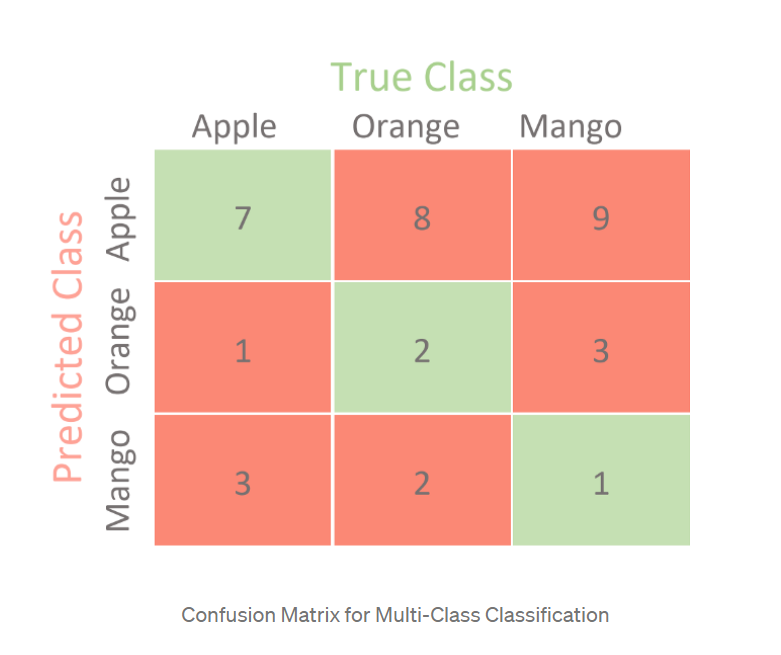
\includegraphics{confusion_matrix.png}

\textit{Figure 1: Confusion matrix example}
\end{center}

\noindent The diagonal elements of the confusion matrix are the occurences where the predictions matched the target values. We can use the confusion matrix to generate other metrics such as precision.


\vspace{3mm}
\noindent
\textbf{Precision}

\vspace{3mm}
\noindent
The precision of a given class is \textit{the number of times that class was correctly predicted divided by the total number of predictions for that particular class}:

\[P = \frac{TP}{TP + FP}\]

\noindent
This metric is particularly valuable if we know the value of predicting various features. If predicting a certain column is particularly important we can compute the precision of our model on that column and assess our model in that way. Using the confusion matrix we can extract the total number of predictions for a given feature by summing along that prediction row. We can easily extract the number of accurate predictions for feature $i$ by considering the $i$-th column in the $i$-th row. 

\vspace{3mm}
\noindent
If we want to minimize the number of false positives for a given target we will want to maximize the precision of our model. 


\vspace{3mm}
\noindent
\textbf{Recall}

\vspace{3mm}
\noindent
The recall of a given class is \textit{the number of times that class was correctly predicted divided by the total number of times that class was actually true}:

\[R = \frac{TP}{TP + FN}\]

\noindent
We can obtain this metric by extracting the diagonal element associated with the $i$-th row in question and dividing by the sum along the $i$-th column. 

\vspace{3mm}
\noindent
If we want to minimize the number of false negatives for a given target we will want to maximize the recall of our model. 


\vspace{3mm}
\noindent
\textbf{F-Measure}


\vspace{3mm}
\noindent
The F-Measure combines precision and recall for a given feature into one metric. A model that has excellent precision and excellent recall will have an F-Measure that approaches 1. A model with weak precision or weak recall will have a resultant F-Measure that is closer to 0. To calculate the F-Measure of a feature we use the following formula:

\[F = \frac{2 \cdot P \cdot R}{P + R}\]


% \section{Feature Selection}
% \subsection{SciKit Learn}
% SciKit Learn allows us to quickly select features based on a wide variety of univariate statistical tests. We can remove all but the $k$ highest scoring features or all but the features in a pre-defined user-specified percentage of features subject to a statistical test (e.g. $\chi^2$). 


% \section{Model Validation}
% \subsection{Performance Metrics}

% \subsection{Multi-Class Classification}
% Using the softmax function we can generate probabilistic predictions. We can then choose to penalize these predictions in any way we see fit. Naively, we can consider the accuracy calculated by taking the sum of all of the correct predictions and dividing by the total number of predictions. Unfortunately, this metric does not make distinctions between classes. A correct answer for 'Class A' is weighted the same as a correct answer for 'Class B' and 'Class C'. But what if there are 100 'Class A' targets and only 5 'Class B' and 'Class C' targets? A model that never predicted 'Class C' or 'Class B' would do well. 

% \subsubsection{Micro Multi-Class Accuracy}
% To compute this accuracy we calculate the total number accurate predictions for each class and then divide by the total number of false predictions for each class. 

% \subsubsection{Micro vs. Macro Metrics}
% If we have a dataset with balanced data then the accuracy metric that we use isn't entirely relevant. Since the target variable has a similar number of elements for each category biasing towards the categories with more elements doesn't have much of an impact.

% \vspace{3mm}
% \noindent
% If our dataset has a significant imbalance in the target variable then we have to decide whether we want a model that is biased towards the most populated targets or whether we want a model that is biased to the least populated targets (and as a result, is not biased towards the most populated targets). This choice is situational and is dependent not on the data, but on the context surrounding the data. 

% If we wish to bias our model to more populated targets we choose a micro metric. Conversely, if we wish to bias our model to less populated targets we choose a macro metric. 

% \subsubsection{}


% % \begin{lstlisting}[language=Python, caption=Python example]
% %     import numpy as np
        
% %     def incmatrix(genl1,genl2):
% %         m = len(genl1)
% %         n = len(genl2)
% %         M = None #to become the incidence matrix
% %         VT = np.zeros((n*m,1), int)  #dummy variable
        
% %         #compute the bitwise xor matrix
% %         M1 = bitxormatrix(genl1)
% %         M2 = np.triu(bitxormatrix(genl2),1) 
    
% %         for i in range(m-1):
% %             for j in range(i+1, m):
% %                 [r,c] = np.where(M2 == M1[i,j])
% %                 for k in range(len(r)):
% %                     VT[(i)*n + r[k]] = 1;
% %                     VT[(i)*n + c[k]] = 1;
% %                     VT[(j)*n + r[k]] = 1;
% %                     VT[(j)*n + c[k]] = 1;
                    
% %                     if M is None:
% %                         M = np.copy(VT)
% %                     else:
% %                         M = np.concatenate((M, VT), 1)
                    
% %                     VT = np.zeros((n*m,1), int)
        
% %         return M
% % \end{lstlisting}

\end{document}